\section{Outil développé}\label{ssec:outil_develope}
\subsection{Procédure suggérée de création d'inventaire}
Le logigramme \ref{fig:logigramme_procédural} montre la procédure générale de création de l'inventaire que devrait entreprendre un analyste pour obtenir un inventaire. Comme tout processus de génération d'ensembles de données, le processus est itératif et requiert des mises à jour pour améliorer l'estimé ainsi qu'une mise à jour avec de nouvelles constructions.
\begin{figure}[!h]
            \centering
            \begin{tikzpicture}
                \tikzstyle{startstop} = [rectangle, rounded corners, minimum width=2cm, minimum height=0.7cm,text centered, draw=black, fill=red!30]
                \tikzstyle{io} = [trapezium, trapezium left angle=70, trapezium right angle=110, minimum width=2cm, minimum height=0.7cm, text centered, draw=black, fill=blue!30,text width=3cm]
                \tikzstyle{process} = [rectangle, minimum width=3cm, minimum height=0.7cm, text centered, draw=black, fill=orange!30,text width=4cm]
                \tikzstyle{database} = [cylinder, text centered, draw=black, fill=yellow!30, shape border rotate = 90, aspect=0.1, text width = 3cm]
                \tikzstyle{decision} = [diamond, minimum width=3cm,  text centered, draw=black, fill=green!30, aspect=2]
                \tikzstyle{arrow} = [thick,->,>=stealth]
                % Nodes de flowchart
                \node (start) [startstop] {Début};
                \node (creation_historique) [process, below right of=start,yshift=-1cm,xshift=2cm] {Création / modification de l'historique de la municipalité}; 
                \node (televerse_secteurs) [process, below of=creation_historique,yshift=-1cm] {Téléversement des limites géographiques des municipalités}; 
                \node (televerse_role)[process, left of=creation_historique,xshift=-4.5cm] {Téléversement des données foncières};
                \node (assoc_cadastre_role)[process, below of=televerse_role,yshift=-0.75cm] {Création / modification association cadastre - rôle foncier};
                \node (televerse_cubf)[process, below of=assoc_cadastre_role,yshift=-0.75cm] {Téléversement de la liste des \ac{CUBF}};
                \node (donnees_pretes)[decision,below of=start,yshift=-6cm,text width=2cm]{Données prêtes?};
                \node (creation_unites)[process, below of=donnees_pretes,yshift=-1.5cm,text width=7cm]{Création / modification des conversions d'unités};
                \node (creation_reglement)[process,below of=creation_unites,yshift=-1.25cm,text width=7cm]{Création / modification des règlements pour les différentes municipalités};
                \node (creation_ens_reg)[process,below of=creation_reglement,yshift=-1cm,text width=7cm]{Création / modification des ensembles de règlements};
                \node (association_ens_reg_terr)[process,right of=creation_ens_reg,xshift=7cm,text width=5cm]{Création / modification association ensembles règlements aux territoires};
                \node (creation_inventaire)[process,above of=association_ens_reg_terr,yshift=0.75cm,text width=5cm]{Création / modification de l'inventaire};
                \node (identification_lots_mal_estimes)[process,above of=creation_inventaire,yshift=0.5cm,text width=5cm]{Identification lots mals estimés};
                \node (tous_lots_estimes)[decision,above of=identification_lots_mal_estimes,yshift=1.25cm,text width=3cm]{Lots estimés et valides?};
                \node (validation_inventaire)[process,above of=tous_lots_estimes,yshift=1cm,text width=5cm]{Validation de l'inventaire};
                \node (aggreg_data_neighbourhood)[process,above of=validation_inventaire,yshift=0.25cm,text width=5cm]{Aggrégation de l'inventaire à l'échelle d'un quartier};
                \node (analyse_critique)[process,above of=aggreg_data_neighbourhood,yshift=0.5cm,text width=5cm]{Analyse critique des résultats};
                \node (vraisemblable)[decision,above of=analyse_critique,yshift=1cm,text width=3cm]{Vraisemblable?};
                \node (fin)[startstop,above of=vraisemblable,yshift=1cm]{Fin};
                \draw [arrow] (start.east) -| (creation_historique.north);
                \draw [arrow] (start.west) -| (televerse_role.north);
                \draw [arrow] (creation_historique) -- (televerse_secteurs);
                \draw [arrow] (televerse_secteurs.south) |-  (donnees_pretes.east);
                \draw [arrow] (televerse_role) -- (assoc_cadastre_role);
                \draw [arrow] (assoc_cadastre_role) -- (televerse_cubf);
                \draw [arrow] (televerse_cubf) |- (donnees_pretes);     
                \draw [arrow] (donnees_pretes.south) -- ++(0,-0.25) node[anchor=west]{O}-- (creation_unites);   
                \draw [arrow] (donnees_pretes.north) -- ++(0,0.5) node[anchor=west] {N} -- (start);   
                \draw [arrow] (creation_unites) -- (creation_reglement);
                \draw [arrow] (creation_reglement) -- (creation_ens_reg);
                \draw [arrow] (creation_ens_reg) -- (association_ens_reg_terr);
                \draw [arrow] (tous_lots_estimes.west) -| ++(-0.250,0) node[anchor=north] {N} |- (creation_historique.east);
                \draw [arrow] (association_ens_reg_terr.north) -- (creation_inventaire);
                \draw [arrow] (creation_inventaire) -- (identification_lots_mal_estimes);
                \draw [arrow] (identification_lots_mal_estimes) -- (tous_lots_estimes);
                \draw [arrow] (tous_lots_estimes.north) -- ++(0,0.1cm) node[anchor=west]{O} -- (validation_inventaire);
                \draw [arrow] (validation_inventaire) -- (aggreg_data_neighbourhood);
                \draw [arrow] (aggreg_data_neighbourhood)-- (analyse_critique);
                \draw [arrow] (analyse_critique)--(vraisemblable);
                \draw [arrow] (vraisemblable.west) -| ++(-0.5,2.25cm) node[anchor=south]{N}  |- ++(-0.5,0)-|(start.north);
                \draw [arrow] (vraisemblable.north)-- ++(0,0.25) node [anchor=west]{O}--(fin);
            \end{tikzpicture}
            \caption{Procédure de génération de l'inventaire}
            \label{fig:logigramme_procédural}
        \end{figure}
\subsection{Fonctions de l'API serveur}
Il est ensuite possible de formuler l'ensemble des requêtes que l'on veut potentiellement remplir et montrer sur la machine \og{client} \fg{}. L'implémentation proposée reprend librement le standard \ac{REST} \parencite{fielding_architectural_2000} qui transmet les requêtes et les réponses au moyen du protocole \ac{HTTP}. Ce type d'interface a typiquement 4 grandes fonctions: GET, PUT, POST, DELETE. GET sert à obtenir un élément de la base de données. PUT permet de modifier un élément déjà existant. POST permet de créer un nouvel élément dans une table. DELETE sert à supprimer un élément. Le chemin auquel ces instructions sont transmises détermine quelle table dans la base de données est consultée ou modifiée. Dans les prochaines sections, une liste sera dressée des variations de GET/PUT/POST/DELETE et d'\ac{URI} implémentés dans le cadre de ce mémoire.
\subsubsection{Inventaire} 
Les appels d'API suivants sont proposés pour les objets de type inventaire:
\begin{itemize}
    \item GET /api/inventaire/quartier/$<id_{quartier}>$: Renvoie l'inventaire pour un quartier complet
    \item GET /api/inventaire/calcul/quartier/$<id_{quartier}>$: renvoie le résultat du calcul détaillé dans la section \ref{sec:meth_urb_based_inventory} pour un quartier d'analyse
    \item GET /api/inventaire/calcul/lot/$<g\_no\_lot>$: renvoie le résultat du calcul détaillé dans la section \ref{sec:meth_urb_based_inventory} pour un lot cadastral. Pour l'ensemble des identifiants de lots cadastraux, les espaces dans le numéro de lot sont remplacés par des tirets bas. Ce remplacement est nécessaire pour éviter de mettre des espaces dans l'\ac{URL}.
    \item POST /api/inventaire/calcul/reg-val-man permet de faire un calcul pour des valeurs manuellement entrées par l'utilisateur. Les valeurs manuelles sont transmises dans le corps de la requête. Les entrées suivantes doivent être présentes pour chaque entrée:
    \begin{itemize}
        \item g\_no\_lot: l'identifiant de lot
        \item cubf: le code d'utilisation du bien fond applicable
        \item id\_reg\_stat: l'identifiant de règlement pertinent
        \item id\_er: l'identifiant d'ensemble de règlement pertinent
        \item unite: l'identifiant d'unité de la valeur fournie
        \item valeur: la valeur manuelle entrée par l'utilisateur
    \end{itemize}
    \item PUT /api/inventaire/$<id_{inv}>$: Modification de l'entrée dans la table \ul{inventaire\_ stationnement} dont l'identifiant est égal à la valeur entre <>. Le contenu de l'entrée est communiqué dans le corps du message avec les variables suivantes:
    \begin{itemize}
        \item g\_no\_lot
        \item n\_places\_min
        \item n\_places\_max
        \item n\_places\_mesure
        \item n\_places\_estime
        \item id\_er
        \item id\_reg\_stat
        \item commentaire
        \item methode\_estime
        \item cubf
    \end{itemize}
    \item POST /api/inventaire: nouvelle entrée dans la table \underline{inventaire\_stationnement}. Les informations suivantes sont fournies dans le corps du message:
    \begin{itemize}
        \item g\_no\_lot
        \item n\_places\_min
        \item n\_places\_max
        \item n\_places\_mesure
        \item n\_places\_estime
        \item id\_er
        \item id\_reg\_stat
        \item commentaire
        \item methode\_estime
        \item cubf
    \end{itemize}
    \item DELETE /api/inventaire/$<id_{inv}>$: supprime l'entrée dont l'id\_inv est égal à la valeur entre <>.
\end{itemize}\clearpage

\subsubsection{Règlements}
Les appels d'\ac{API} suivants sont proposés pour les objets de type règlement:
\begin{itemize}
    \item GET /api/reglements/entete: renvoie toutes les entêtes de règlements (description, information administrative)
    \item GET /api/reglements/<id\_reg\_stat>: renvoie l'ensemble du règlement dont l'identifiant est égal à celui fourni par l'utilisateur
    \item PUT /api/reglements/<id\_reg\_stat>: modifie le règlement dont l'identifiant est égal à id\_reg\_stat. Les paramètres à fournir sont les suivants. Ces paramètres suivent les définitions de types montrées au Tableau \ref{tab:definition_entete_reg_stationnement} et \ref{tab:definition_reg_stat_emp}.
        \begin{itemize}
            \item entete:
                \begin{itemize}
                    \item id\_reg\_stat
                    \item description
                    \item annee\_debut\_reg
                    \item annee\_fin\_reg
                    \item texte\_loi
                    \item article\_loi
                    \item paragraphe\_loi
                    \item ville
                \end{itemize}
            \item definition, un tableau dont les colonnes sont:
                \begin{itemize}
                    \item id\_reg\_stat\_emp
                    \item id\_reg\_stat
                    \item ss\_ensemble
                    \item seuil
                    \item oper
                    \item cases\_fix\_min
                    \item cases\_fix\_max
                    \item pente\_min
                    \item pente\_max
                    \item unite
                \end{itemize}
        \end{itemize}
    \item POST /api/reglements permet de créer un nouveau règlement et requiert les mêmes informations que la fonction PUT mais n'a pas d'identifiant dans l'\ac{URL}.
\end{itemize}\clearpage
\subsubsection{Ensembles de règlements}
Les appels d'\ac{API} suivants sont proposés pour les ensembles de règlements.
\begin{itemize}
    \item GET /api/ens-reg/entete renvoie l'ensemble des entêtes de règlements de stationnement dont les propriétés sont listées dans le Tableau \ref{tab:definition_er}:
    \begin{itemize}
        \item id\_er 
        \item date\_debut\_er
        \item date\_fin\_er
        \item description\_er
    \end{itemize}
    \item GET /api/ens-reg/complet/<id\_er> renvoie  les données suivantes pour l'ensemble de règlement dont l'identifiant est égal à id\_er:
        \begin{itemize}
            \item entete
                \begin{itemize}
                    \item id\_er
                    \item date\_debut\_er
                    \item date\_fin\_er
                    \item description\_er
                \end{itemize}
            \item assoc\_util\_sol
                \begin{itemize}
                    \item id\_assoc\_er\_reg identifiant primaire
                    \item id\_reg\_stat, l'identifiant du règlement
                    \item cubf, le \ac{CUBF} pour l'utilisation du sol
                    \item id\_er, l'identifiant d'ensemble règlement
                \end{itemize}
            \item table\_util\_sol
                \begin{itemize}
                    \item \ac{CUBF}
                    \item description
                \end{itemize}
        \end{itemize}
    
    \item PUT /api/ens-reg/complet/<id\_er> modifie un ensemble de règlements existant. Les données suivantes doivent être fournies dans le corps:
        \begin{itemize}
            \item entete
                \begin{itemize}
                    \item date\_debut\_er
                    \item date\_fin\_er
                    \item description\_er
                \end{itemize}
            \item assoc\_util\_sol
                \begin{itemize}
                    \item id\_assoc\_er\_reg identifiant primaire
                    \item id\_reg\_stat, l'identifiant du règlement
                    \item cubf, le \ac{CUBF} pour l'utilisation du sol
                \end{itemize}
        \end{itemize}
    \item GET /api/ens-reg/reg-associes/<id\_er> renvoie les entêtes des règlements qui sont utilisés dans l'ensemble de règlements dont l'identifiant est égal à id\_er.
    \item GET /api/ens-reg/entete-par-territoire/<id\_periode\_geo> renvoie les entêtes des ensembles de règlements associés au territoire dont l'identifiant est égal à id\_periode\_geo.
    \item POST /ens-reg/complet permet de créer un nouvel ensemble de règlements en utilisant les mêmes informations que celles listées pour PUT. L'id\_er doit cependant être omis des propriétés et est attribué dans la procédure de création.
        \begin{itemize}
            \item entete
                \begin{itemize}
                    \item date\_debut\_er
                    \item date\_fin\_er
                    \item description\_er
                \end{itemize}
            \item assoc\_util\_sol
                \begin{itemize} 
                    \item id\_assoc\_er\_reg identifiant primaire
                    \item id\_reg\_stat, l'identifiant du règlement
                    \item cubf, le \ac{CUBF} pour l'utilisation du sol
                \end{itemize}
        \end{itemize}
    \item DELETE /api/ens-reg/complet/<id\_er> permet de supprimer un ensemble de règlements. Le serveur s'assure que cet ensemble n'est pas utilisé dans un ensemble de règlements-territoire avant de supprimer.
    \item PUT /api/ens-reg/assoc/<id\_assoc\_er\_reg> permet de modifier une association spécifique dans un ensemble de règlements. Les champs décrits dans le tableau \ref{tab:definition_association_er_reg_stat}. Les entrées ayant un \ac{CUBF} entre 1 et 9 ne peuvent modifier que le règlement. En effet, au minimum, un ensemble de règlements doit contenir les CUBF 1 à 9. Les variables suivantes doivent être fournies dans le corps de la requête
    \begin{itemize}
        \item id\_reg\_stat, l'identifiant du règlement
        \item cubf, le \ac{CUBF} pour l'utilisation du sol
        \item id\_er, l'identifiant d'ensemble règlement
    \end{itemize}
    \item POST /api/ens-reg/assoc permet de créer une nouvelle association entre un \ac{CUBF} et un règlement. Les variables du tableau \ref{tab:definition_association_er_reg_stat} doivent être fournies:
    \begin{itemize}
        \item id\_reg\_stat, l'identifiant du règlement
        \item cubf, le \ac{CUBF} pour l'utilisation du sol
        \item id\_er, l'identifiant d'ensemble règlement
    \end{itemize}
    \item DELETE /api/ens-reg/assoc/<id\_assoc\_er\_reg> permet de supprimer l'association dont l'identifiant est fourni dans l'\ac{URL}.
\end{itemize}\clearpage
\subsubsection{Territoire}
L'\ac{API} possède les appels suivants pour manipuler les territoires:
\begin{itemize}
    \item GET /api/territoire/periode/<id\_periode> permet d'obtenir l'ensemble des territoires associés qui sont associés à la période spécifiée dans l'\ac{URL}.
    \item GET /api/territoire/periode-geo/<id\_periode\_geo> permet d'obtenir un territoire selon son identifiant unique.
    \item PUT /api/territoire/periode-geo/<id\_periode\_geo> permet de mettre à jour un territoire.
    \item POST /api/territoire/periode/<id\_periode> permet d'ajouter des territoires associés à une période. Les colonnes suivantes devront être fournies dans le corps du message en concordance avec les types définis dans le tableau \ref{tab:definition_cartographie_secteurs}:
    \begin{itemize}
        \item id\_periode, l'identifiant de la période à laquelle est associée 
        \item ville
        \item secteur
        \item ville\_sec
        \item geometry, la géométrie sous format WKT en CRS 4326
    \end{itemize}
    \item POST /api/territoire/periode-geo permet d'ajouter un territoire à la cartographie. Les colonnes suivantes doivent être fournies dans le corps de la requête:
    \begin{itemize}
        \item id\_periode, l'identifiant de la période à laquelle est associée 
        \item ville
        \item secteur
        \item ville\_sec
        \item geometry, la géométrie sous format WKT en CRS 4326
    \end{itemize}
    \item DELETE /api/territoire/periode-geo/<id\_periode\_geo> permet de supprimer des territoires en fonction de l'identifiant du territoire
\end{itemize}
\clearpage
\subsubsection{Historique}
L'\ac{API}  possède les appels suivants pour manipuler l'historique de la ville:
\begin{itemize}
    \item GET /api/historique obtient l'ensemble des entrées de la table \ul{historique\_geopol} avec les entrées du Tableau \ref{tab:definition_historique_geopol}
    \item GET /api/historique/<$id_{periode}$> renvoie un item de la table \ul{historique\_geopol} dont l'identifiant est égal à $id_{periode}$
    \item PUT /api/historique/<$id_{periode}$> permet de modifier un item de la table \ul{historique\_ geopol}. Les colonnes suivantes doivent être dans le corps du message selon les types 
    \begin{itemize}
        \item nom\_periode 
        \item date\_debut\_periode
        \item date\_fin\_periode
    \end{itemize}
    \item POST /api/historique permet de créer une nouvelle période dans la base de données. Les colonnes suivantes doivent être dans le corps du message.
    \begin{itemize}
        \item nom\_periode 
        \item date\_debut\_periode
        \item date\_fin\_periode
    \end{itemize}
    \item DELETE /api/historique/<$id_{periode}$> permet de supprimer la période dont l'identifiant est égal à $id_{periode}$
\end{itemize}


\subsubsection{Lots cadastraux et entrées du rôle foncier}
Les appels d'\ac{API} suivants ont été implémentés pour les lots cadastraux et les entrées du rôle:
\begin{itemize}
    \item GET /api/cadastre/lot/quartier-ana/<$id_{quartier}$> permet d'obtenir l'ensemble des lots qui se situent à l'intérieur du quartier d'analyse dont l'identifiant est fourni dans l'\ac{URI}
    \item GET /api/cadastre/lot/<$g\_no\_lot$> permet d'obtenir le lot dont l'identifiant est égal à la valeur fournie de g\_no\_lot. Comme pour les autres appels reliés à un lot cadastral, les espaces doivent être remplacés par un tiret bas dans l'\ac{URL}.
    \item GET /api/cadastre/role-associe/<$g\_no\_lot$> permet d'obtenir les entrées du rôle foncier 
    \item POST /api/cadastre/cadastre permet de créer un nouveau lot cadastral
    \item POST /api/cadastre/role permet de créer une nouvelle entrée au rôle foncier
    \item POST /api/cadastre/cadastre/en-gros permet de créer plusieurs nouvelles entrées dans la table \ul{cadastre} dont les colonnes sont détaillées au Tableau \ref{tab:definition_cadastre}
    \item POST /api/cadastre/role/en-gros permet de créer de nouvelles entrées dans la table \ul{role\_foncier} dont les colonnes sont détaillées au Tableau \ref{tab:definition_role_foncier}
    \item GET /api/cadastre/creer-association permet d'obtenir le résultat de la jointure spatiale entre les points du rôle foncier et les polygones du cadastre. 
    \item POST /api/cadastre/association permet de créer une nouvelle entrée dans la table \ul{association\_cadastre\_role} dont les colonnes sont détaillées au Tableau \ref{tab:definition_assoc_role_cadastre}. Seules les colonnes id\_provinc et g\_no\_lot doivent être spécifiées dans le corps de la requête.
    \item PUT /api/cadastre/association/<$id_{assoc}$> permet de modifier l'association dont l'identifiant est spécifié dans l'\ac{URL}. Comme pour l'opération POST, seules les colonnes id\_ provinc et g\_ no\_lot doivent être spécifiées dans le corps de la requête.
    \item DELETE /api/cadastre/association/<$id_{assoc}$> permet de supprimer l'association dont l'identifiant est spécifiée dans la l'\ac{URL}
\end{itemize}
\subsubsection{Facteurs de conversion}
Les appels d'\ac{API} suivants doivent être mis en place pour gérer la table \ul{multiplicateur\_ facteurs\_colonnes} qui est décrite au tableau \ref{tab:definition_unite}
\begin{itemize}
    \item GET /api/conversions/ permet d'obtenir l'ensemble des entrées de la table \ul{multiplicateur\_ facteurs\_colonnes}
    \item GET /api/conversions/<$id_{unite}$> permet d'obtenir l'entrée dont la variable identifiant d'unité est spécifié dans l'\ac{URL}
    \item PUT /api/conversions/<$id_{unite}$> permet de modifier l'entrée dont l'identifiant d'unité est spécifié dans l'\ac{URL}. Les variables colonne\_role\_foncier, facteur\_correction, desc\_unite et ordonnee\_ correction doivent être fournies dans le corps de la requête.
    \item POST /api/conversions/ permet de créer une nouvelle entrée dans la table et les variables doivent être fournies dans le corps de la requête.
    \item DELETE /api/conversions/<$id_{unite}$> supprime l'entrée dans la table dont l'identifiant est fourni dans l'\ac{URL}
\end{itemize}
\subsubsection{Secteurs d'analyse}
L'\ac{API} permet de manipuler les secteurs municipaux utilisés pour l'analyse qui sont définis à la section \ref{ssec:struct_donnees_sec_analyse}.
\begin{itemize}
    \item GET /api/quartiers-analyse obtient l'ensemble des quartiers dans la table \ul{sec\_analyse}
    \item PUT /quartiers-analyse/<$id_{quartier}$> modifie une entrée. Les propriétés suivantes doivent être dans le corps de la requête selon les types du tableau \ref{tab:definition_sec_analyse}.
        \begin{itemize}
            \item nom\_quartier
            \item superf\_quartier la superficie du quartier en mètre carrés
            \item peri\_quartier le périmètre du quartier en mètres
            \item geometry, la géométrie du quartier en format WKT en CRS 4326
        \end{itemize}
    \item POST /api/quartiers-analyse permet de créer un nouveau quartier. Les propriétés suivantes doivent être dans le corps de la requête :
        \begin{itemize}
            \item nom\_quartier
            \item superf\_quartier la superficie du quartier en mètre carrés
            \item peri\_quartier le périmètre du quartier en mètres
            \item geometry, la géométrie du quartier en format WKT en CRS 4326
        \end{itemize}
    \item POST /api/quartiers-analyse/en-gros permet de créer plusieurs quartiers. Les propriétés suivantes doivent être dans le corps de la requête.
        \begin{itemize}
            \item nom\_quartier
            \item superf\_quartier la superficie du quartier en mètre carrés
            \item peri\_quartier le périmètre du quartier en mètres
            \item geometry, la géométrie du quartier en format WKT en CRS 4326
        \end{itemize}
    \item DELETE /api/quartiers-analyse/<$id_{quartier}$> permet de supprimer une entrée de la table \ul{sec\_analyse}
\end{itemize}
\subsubsection{Profile d'accumulation véhicule}
Les appels d'\ac{API} suivants sont mis en place pour gérer les profils d'accumulation véhicule \parencite{diallo_methodology_2015} qui permettent de trouver la \og{population}\fg{} de véhicules dans une géographie en fonction de l'heure de la journée.
\begin{itemize}
    \item GET /api/PAV?order=X,Y,Z\&id\_quartier=<$id_{quartier}$> permet d'accéder au profile d'accumulation véhicule pour le quartier dont l'identifiant est spécifié. L'ordre spécifié donne l'ordre de préséance pour le relevé de l'inventaire du quartier. En effet, l'APi fournit l'inventaire du quartier en même temps pour visuellement  constater la variation de la capacité au courant de la journée
    \item GET /api/PAV/recalcule/<$id_{quartier}$> permet de refaire le calcul du profile d'accumulation véhicule à partir des données de l'enquête OD
    \item POST /api/PAV/<$id_{quartier}$> permet de mettre à jour le profile d'accumulation dans la base de données une fois que l'utilisateur l'a confirmé
    \item DELETE /api/PAV/<$id_{quartier}$> permet de supprimer le profile d'accumulation dans la base de données
\end{itemize}

\clearpage
\subsection{Pages de l'interface}
Plusieurs pages ont été développées pour permettre à un analyste de visualiser, modifier les intrants et analyser les résultats de l'inventaire. Ces pages seront décrites dans cette section
\subsubsection{Règlements}
La page règlements permet de créer et modifier les différents règlements. La figure \hl{créer figure }montre l'interface. En haut se trouve le menu qui permet de naviguer entre les différentes pages. La partie centrale est une liste des règlements entreposés dans la base de données, en montrant les information entreposées dans l'entête du règlement incluant:
\begin{itemize}
    \item une description du règlement, 
    \item les dates d'entrée en vigueur et d'abrogation du règlement
    \item des information sur le texte de loi, l'article et le paragraphe où sont définis les règlements dans la loi
    \item le nom de la ville d'où vient le règlement. Il est important de noter que le nom de cette ville n'est pas associé aux informations de la géopolitique de la ville mais est simplement là pour référence
\end{itemize}
En cliquant sur un élément dans la liste, l'utilisateur peut accéder à la définition mathématique, telle qu'elle est entreposée dans la base de données.\par
La partie inférieure de l'écran permet de visualiser et modifier la définition du règlement

\subsubsection{Historique}
Comme pour la page des règlements, le haut de la page d'historique est rempli par le menu permettant de naviguer entre les différentes pages de l'outil.\par
Le bandeau gauche manipule l'historique tel que défini dans la table \ul{historique\_geopol} défini au tableau \ref{tab:definition_historique_geopol}. On peut y ajouter des périodes, changer les dates des périodes et le nom des grandes périodes de l'historique. Les années sont inclusives (i.e 2023-2027 inclut les années 2023, 2024, 2025, 2026 et 2027).\par
Le bandeau en bas permet de modifier certaines informations quand au nom de la ville et du secteur. Il est important de noter que les noms des municipalités peuvent être corrigées et des secteurs supprimés mais aucune modification des limites géopolitiques ne peut être complétée. Les limites doivent être ajoutées à partir de fichier GeoJSON.\par
Les secteurs peuvent être supprimés s'ils ne sont pas utilisés dans des \ac{RST}.\par
La carte montre les secteurs et est mise à jour en fonction de la période sélectionnée en même temps que la table dans le tableau en bas de page pour que seuls les territoires associés à la période sélectionnée ne soient montrés.
\begin{landscape}
    \begin{figure}
        \centering
        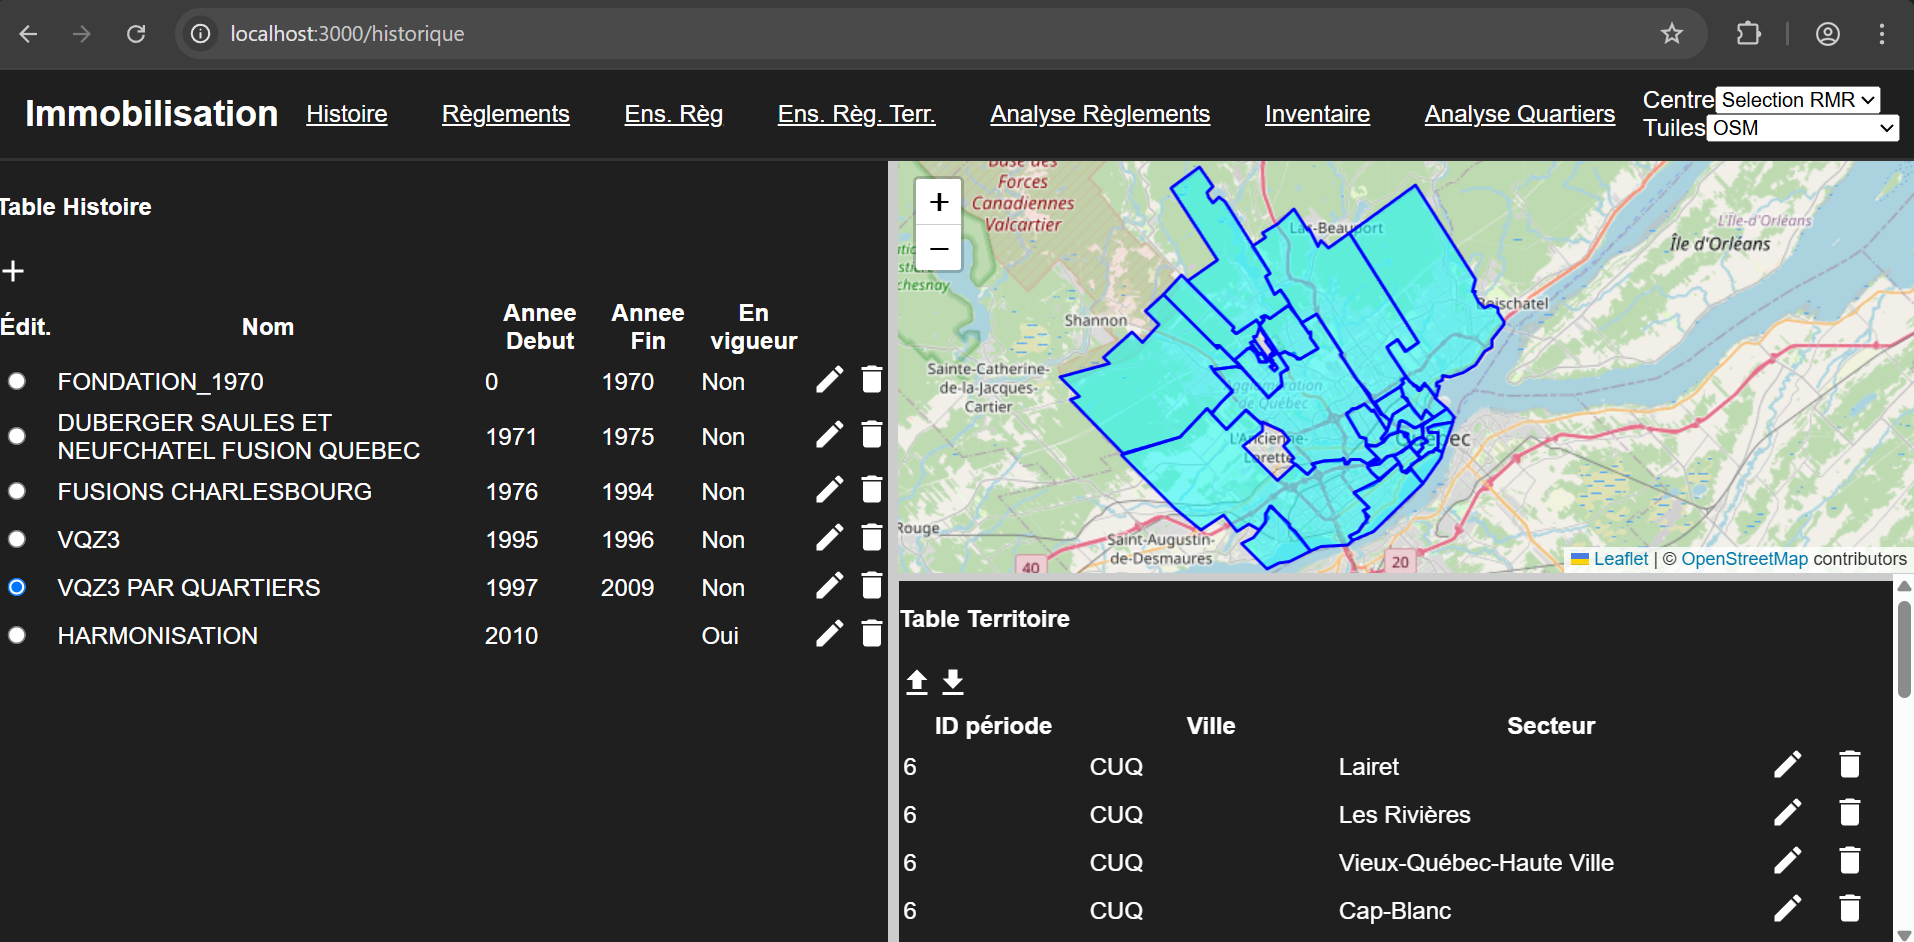
\includegraphics[width=1\linewidth]{images/PageHistorique.png}
        \caption{Page de}
        \label{fig:page_historique}
    \end{figure}
\end{landscape}
\subsubsection{Ensembles de règlements}
La page Ensemble de Règlements permet de modifier les ensembles de règlements. Le bandeau de gauche donne une liste de l'ensemble des ensembles de règlements entreposés dans la table \ul{ensembles\_reglement\_stat}